\documentclass[12pt, final]{extarticle}

% SECTION Paquetes
\usepackage{blindtext}
\usepackage{geometry}
\usepackage{minted}
\usepackage{lmodern}
\usepackage{caption}
\usepackage{subcaption}
\usepackage[spanish]{babel}
\usepackage[T1]{fontenc}
\usepackage{csquotes}
\usepackage{amsmath}
\usepackage{gensymb}
\usepackage[dvipsnames]{xcolor}
\usepackage{graphicx}
\usepackage[hidelinks]{hyperref}

% SECTION Configuraciones y macros
\geometry{top=3cm, bottom=2.8cm, left=2.6cm, right=2.6cm}

\graphicspath{{Media}}

\definecolor{bg}{gray}{0.97}
\usemintedstyle{manni}
\setminted{linenos, frame=lines, bgcolor=bg}

\renewcommand{\abstractname}{Resumen}

% SECTION Datos del título
\title{ADA 5\\
\textsc{Animación y Simulación del Mecanismo 4R-3E}}
\author{J. Ayil, C. Canul, E. Chablé, F. Sánchez, S. Tuyú\\
{Facultad de Ingeniería, Universidad Autónoma de Yucatán}}
\date{}

% SECTION Comenzar documento
\begin{document}
\maketitle

\begin{abstract}
   En esta actividad se encuentra un análisis general del mecanismo de cuatros barras con tres engranajes, en donde se establece de manera detallada el análisis cinemático con el método vectorial y el trigonométrico, asi como, la simulación y animación del mecanismo 4R-3E con ambos métodos, todo ello hecho por medio del software MatLab. 
\end{abstract}

\section{Análisis cinemático}
\subsection{Método trigonométrico}
\begin{figure}[ht]
    \centering
    \begin{subfigure}[b]{0.45\textwidth}
        \centering
        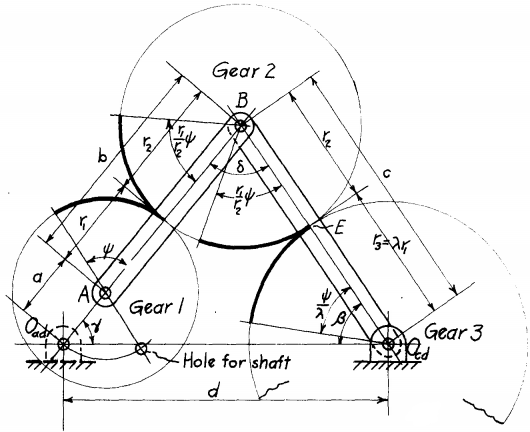
\includegraphics[width=\textwidth]{MT_1a}
        \caption{}
        \label{Fig: Los tres engranajes de transmision a}
    \end{subfigure}
    \hfill
    \begin{subfigure}[b]{0.45\textwidth}
        \centering
        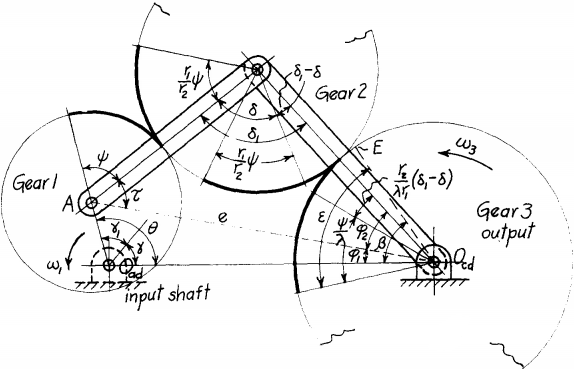
\includegraphics[width=\textwidth]{MT_2a}
        \caption{}
        \label{Fig: Los tres engranajes de transmision b}
    \end{subfigure}
    \caption{Los tres engranajes de transmisión.}
    \label{Fig: Los tres engranajes de transmision}
\end{figure}

Cuando las barras $a$ y $b$ están en una línea recta como se muestra en la
figura \ref{Fig: Los tres engranajes de transmision a}, los ángulos del
triángulo resultante son $\beta$, $\gamma$ y $\delta$. Deje
\begin{equation}
    s = \frac{1}{2}(a + b + c + d)
\end{equation}
Por trigonometría
\begin{align}
    \cos^2 \frac{\delta}{2} &= \frac{s(s - d)}{(a + b)c} \\
    \cos \delta &= 2\cos^2 \frac{\delta}{2} - 1 = \frac{2s(s - d)}{(a + b)c} - 1
\end{align}
Por teorema de senos
\begin{align}
    \sin \gamma &= \frac{c}{d}\sin\gamma \\
    \beta &= 180\degree - (\gamma + \delta)
\end{align}

Con las uniones en las posiciones de la figura
\ref{Fig: Los tres engranajes de transmision a}, deje que el eje de
transmisión en $O_{ad}$ sea removido, y deje al engrane 1 ser rotado a través
del ángulo $\psi$. Esto produce rotaciones en los engranes 2 y 3 como se indica
por los arcos gruesos y los ángulos designados.

Deje que los engranes 1 y 2 sean unidos al miembro $ab$, y deje que el mecanismo
sea movido de tal manera que el eje de transmisión pueda ser reconstruido en
$O_{ad}$. Las partes ahora están en los lugares mostrados en la figura
\ref{Fig: Los tres engranajes de transmision b} con el eje de transmisión
girado a través del ángulo $\gamma_{1}$. El ángulo $\delta$ es aumentado hasta
$\delta_{1}$, y la inclinación de la unión $BO_{cd}$ es cambiada por el valor
$\beta - (\phi_{1} + \phi_{2})$. Los engranes 2 y 3 sufrieron una rotación
adicional.

La ecuación para la rotación $\epsilon$ del engrane 3 es el que se presenta a
continuación.
\begin{equation}
    \theta = \gamma + \gamma_{1}
\end{equation}
Por el teorema de cosenos
\begin{equation}
    e^2 = a^2 + d^2 - 2ad\cos\theta = b^2 + c^2 - 2bc\cos\delta_{1}
\end{equation}
o
\begin{equation}
    \cos\delta_{1} = \frac{b^2 + c^2 - a^2 - d^2}{2bc} + \frac{ad}{bc}\cos\theta
    = K_{1} + K_{2}\cos\theta
    \label{Eq: cos delta1}
\end{equation}
donde
\begin{align}
    K_{1} &= \frac{b^2 + c^2 - a^2 - d^2}{2bc} \\
    K_{2} &= \frac{ad}{bc} \\
    \sin\tau &= \frac{c}{e}\sin\delta_{1} \\
    \phi_{2} &= 180 - (\delta_{1} + \tau) \\
    \sin\phi_{1} &= \frac{a}{e}\sin\theta \\
    \psi &= \theta + \phi_{1} - \tau_{1}
\end{align}
Entonces
\begin{equation}
    \epsilon = \beta - (\phi_{1} + \phi_{2})
    + \frac{r_{2}}{\lambda r_{1}}(\delta_{1} - \delta) + \frac{\psi}{\lambda}
\end{equation}

Para el caso en el que los engranes 1 y 3 tienen el mismo tamaño, $\lambda=1$,
la ecuación para $\epsilon$ se convierte
\begin{equation}
    \epsilon = \theta - \gamma - C\delta + C\delta_{1}
    \label{Eq: epsilon theta menos gamma}
\end{equation}
donde
\begin{equation}
    C = 1 + \frac{r_{2}}{r_{1}}
\end{equation}

Valores de $\epsilon$ pueden ser computador y graficados con estas ecuaciones.

\eqref{Eq: epsilon theta menos gamma} puede ser diferenciada para encontrar la
velocidad $\omega_{3}$ del eje de salida
\begin{equation*}
    \frac{d\epsilon}{dt} = \frac{d\theta}{dt} + C\frac{d\delta_{1}}{dt}
\end{equation*}
El coeficiente diferencial $\frac{d\theta}{dt}$ es igual a $\omega_{1}$, y el
coeficiente diferencial $\frac{d\delta_{1}}{dt}$ puede ser obtenido de
\eqref{Eq: cos delta1}. Entonces
\begin{equation}
    \omega_{3} = \omega_{1} \left[
        1 + \frac{K_{2}C\sin\theta}{\sin\delta_{1}}
    \right]
    \label{Eq: omega3 antes de sustituir}
\end{equation}
y la sustitución de \eqref{Eq: cos delta1} da
\begin{equation}
    \omega_{3} = \omega_{1} \left[
        1 + \frac{K_{2}C\sqrt{1-\cos^2\theta}}{1-(K_{1} + K_{2}\cos\theta)^2}
    \right]
    \label{Eq: omega3 despues de sustituir}
\end{equation}

\eqref{Eq: omega3 antes de sustituir} y \eqref{Eq: omega3 despues de sustituir}
son válidas para el caso en el que $r_{1} = r_{3}$. Diferenciarlas nuevamente
para obtener la aceleración genera una expresión demasiado inmanejable para
aplicaciones prácticas.

La velocidad angular $\omega_{3}$ del eje de salida puede, de igual manera, ser
encontrada por medio de la obtención de la pendiente de los diferentes puntos a
lo largo de la $\epsilon$-curva. Puede ser demostrado\cite{Milne1949} que
cuando las ordenadas $y_{0}$, $y_{1}$, $y_{2}$, $y_{3}$ y $y_{4}$ estén en cinco
equitativamente separados y conocidos puntos, la pendiente $y_{2}$ de la curva
en la ordenada de en medio está dada por la siguiente ecuación.
\begin{equation}
    {y_{2}}' = \frac{1}{12h}(y_{0} - 8y_{1} + 8y_{3} - y_{4})
\end{equation}
donde $h$ es el espaciado a lo largo de la abscisa. El proceso puede ser
repetido en la curva de velocidad para obtener la aceleración angular del eje de
salida.

\newpage
\subsection{Método vectorial}
\begin{figure}[ht]
    \centering
    \begin{subfigure}[b]{0.45\textwidth}
        \centering
        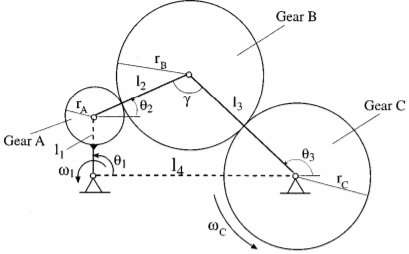
\includegraphics[width=\textwidth]{Media/mecanismo4b-3e.png}
        \caption{}
        \label{Fig: Mecanismo 4B-3E a}
    \end{subfigure}
    \hfill
    \begin{subfigure}[b]{0.45\textwidth}
        \centering
        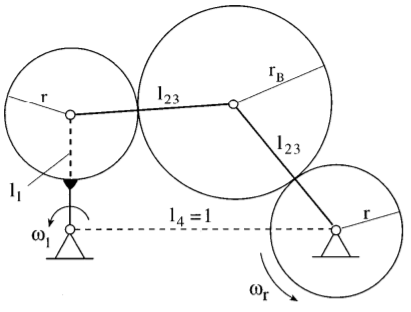
\includegraphics[width=\textwidth]{Media/4B-3E.png}
        \caption{}
        \label{Fig: Mecanismo 4B-3E b}
    \end{subfigure}
    \label{Fig: Mecanismo 4B-3E}
    \caption{Mecanismo 4B-3E.}
\end{figure}

Considere la conexión de tres engranajes que se muestra en la figura \ref{Fig:
Mecanismo 4B-3E a}, donde los desplazamientos angulares de los engranajes son
positivos en sentido anti horario. Al ver el mecanismo como una transmisión
planetaria con el engranaje $B$ como planeta, el eslabón $l_3$ como brazo y el
engranaje $C$ como sol, la condición de rodar sin deslizamiento en el contacto
sol-planeta da:
\begin{equation}
   r_C\theta_C=I_3\theta_3-r_B\theta_B
   \label{Eq: Vect1}
\end{equation}
Notando que:
\begin{equation}
   I_2=r_A+r_B  \quad\quad\quad I_3=r_B+r_C
   \label{Eq: Vect2}
\end{equation}

El desplazamiento del engranaje de salida se obtiene de \eqref{Eq: Vect1},
teniendo:
\begin{equation}
   \theta_C=(1+\frac{r_B}{r_C})(\theta_3-\theta_{30})-\frac{r_B}{r_C}\theta_B
   \label{Eq: Vect3}
\end{equation}

Donde $\theta_{30}=\theta_3(\theta_1=0)$. Para un observador fijo en el enlace
3, la relación de las velocidades angulares relativas del planeta y el sol con
respecto al brazo (que puede considerarse fija) es dado por
\begin{equation}
   \frac{\omega_{B/3}}{\omega_{C/3}}=\frac{\omega_B-\omega_3}{\omega_C-\omega_3}=-\frac{r_C}{r_B}
    \label{Eq: Vect4}
\end{equation}

De \eqref{Eq: Vect4} la velocidad del engranaje de salida se obtiene como
\begin{equation}
   \omega_C=(1+\frac{r_B}{r_C})\omega_3-\frac{r_B}{r_C}\omega_B
   \label{Eq: Vect5}
\end{equation}

Que verifica el desplazamiento \eqref{Eq: Vect3}, siendo su derivada en el tiempo.
De manera similar, para un observador adjunto al eslabón 2, la relación de las
velocidades angulares relativas del engranaje $B$ y el eslabón 1 con respecto al
eslabón 2 viene dada por
\begin{equation}
   \frac{\omega_{B/2}}{\omega_{1/2}}=\frac{\omega_B-\omega_2}{\omega_1-\omega_2}=-\frac{r_A}{r_B}
\end{equation}

Produciendo la velocidad del engranaje B como
\begin{equation}
   \omega_B=(1+\frac{r_A}{r_B})\omega_2-\frac{r_A}{r_B}\omega_1
   \label{Eq: Vect7}
\end{equation}

Reemplazando \eqref{Eq: Vect7} en \eqref{Eq: Vect5} y teniendo en cuenta
\eqref{Eq: Vect2} !, la velocidad del engranaje de salida se convierte en
\begin{equation}
   \omega_C=\frac{1}{r_C}(r_A\omega_1-I_2\omega_2+I_3\omega_3)
   \label{Eq: Vect8}
\end{equation}

A partir de la cinemática de enlace de cuatro \eqref{Eq: Vect7}, $\omega_2$ y
$\omega_3$ se obtienen como
\begin{equation}
   \omega_2=\frac{I_1\sin({\theta_1-\theta_3})}{I_2\sin({\theta_3-\theta_2})}\omega_1  \quad\quad \quad   \omega_3=\frac{I_1\sin({\theta_1-\theta_2})}{I_3\sin({\theta_3-\theta_2})}\omega_1
   \label{Eq: Vect9}
\end{equation}

Donde $\theta_2$ y $\theta_3$ se pueden calcular para un $\theta_1$
especificado. Reemplazando \eqref{Eq: Vect9} en \eqref{Eq: Vect8}, $\omega_C$ se
convierte
\begin{equation}
   \omega_C=\frac{r_A}{r_C}\omega_1+\frac{I_1}{r_C}\omega_1[\frac{\sin({\theta_1-\theta_2})}{\sin({\theta_3-\theta_2})}-\frac{\sin({\theta_1-\theta_3})}{\sin({\theta_3-\theta_2})}]
   \label{Eq: Vect10}
\end{equation}

Nuevamente, a partir de la cinemática del mecanismo de cuatro barras, se puede
demostrar que al satisfacer la condición de dimensionamiento
\begin{equation}
   I_2=I_3=I_{23}
   \label{Eq: Vect11}
\end{equation}

$\theta_2(\theta_1)$ y $\theta_3(\theta_1)$ son funciones pares e impares de
$\theta_1$, respectivamente. Como resultado, el ángulo de transmisión
$\gamma=\theta_3-\theta_2$ de la figura \ref{Fig: Mecanismo 4B-3E a} es una
función par de $\theta_1$, es decir
\begin{equation}
   \gamma(\theta_1)=\gamma(2\pi-\theta_1)
   \label{Eq: Vect12}
\end{equation}

Teniendo en cuenta que \eqref{Eq: Vect11} implica engranajes de entrada y salida
de igual radio (es decir, $\rho=1$), denotamos (Figura \ref{Fig: Mecanismo 4B-3E
b})
\begin{equation}
   r_A=r_C=r\quad\quad\quad \omega_C=\omega_r    \quad\quad\quad \theta_C=\theta_r
   \label{Eq: Vect13}
\end{equation}
y teniendo en cuenta esto en \eqref{Eq: Vect10}, la velocidad del engranaje de
salida toma la forma
\begin{equation}
    \omega_r=\omega_1[1+\frac{I_1}{r}\frac{\sin{(\theta_1-\theta_2)}-\sin{(\theta_1-\theta_3)}}{\sin{\gamma}}]=\omega_1+\Delta\omega
   \label{Eq: Vect14}
\end{equation}

Suponiendo a continuación un movimiento uniforme de la manivela de entrada
\begin{equation}
    \omega_1=\text{const}
   \label{Eq: Vect15}
\end{equation}

Se puede ver desde \eqref{Eq: Vect14} que la variación $\Delta\omega$ con
respecto a $\theta_1$ es periódica e impar, ya que tenemos
\begin{equation}
\Delta\omega(0)=\Delta\omega(180\degree)=0
   \label{Eq: Vect16}
\end{equation}
\begin{equation}
    \Delta\omega(\theta_1+360\degree)=\Delta\omega(\theta_1)  \quad\quad\quad \Delta\omega(360\degree-\theta_1)=-\Delta\omega(\theta_1)
   \label{Eq: Vect17}
\end{equation}

A continuación, a partir de $\omega_r=\theta_r$, el desplazamiento del engranaje
de salida $\theta_r$ se obtiene de \eqref{Eq: Vect8} con \eqref{Eq: Vect11} y
\eqref{Eq: Vect13} como
\begin{equation}
    \theta_r=\theta_1+\frac{I_{23}}{r}[(\theta_3-\theta_2)-(\theta_{30}-\theta_{20})]=\theta_1+\frac{I_{23}}{r}(\gamma-\gamma_0)
   \label{Eq: Vect18}
\end{equation}

Donde la variación pulsatoria de $\gamma$ (con mínimos en $\theta_1=0$ y
$360\degree$ y un máximo en $180\degree$, \eqref{Eq: Vect12}) se superpone a la
variación lineal $\theta_1$. Ahora requerimos que $\Delta\omega$ sea impar y que
tenga una variación con máximo y mínimo en $\theta_1=90\degree$ y $270\degree$
respectivamente. Al observar que $d\Delta\omega/d\theta_1$ depende de $\theta_1$
también a través de $\theta_2$ y $\theta_3$, obtenemos después de algunos
cálculos prolongados la segunda condición de diseño
\begin{equation}
    {I_1}^2+{I_4}^2={I_2}^2+{I_3}^2=2{I_{23}}^2
   \label{Eq: Vect19}
\end{equation}

Las ecuaciones \eqref{Eq: Vect11} y \eqref{Eq: Vect19} representan las
condiciones de dimensionamiento para un enlace de tres engranajes que transforma
una velocidad de manivela de entrada constante $\omega_1$ en una velocidad de
engranaje de salida de tipo sinoidal $\Delta\omega(\theta_1)$ superpuesta a
$\omega_1$. Es interesante notar que \eqref{Eq: Vect11} y \eqref{Eq: Vect19}
también son las condiciones para un mecanismo de cuatro barras "céntrico", donde
la manivela gira $180\degree$ cuando el balancín se mueve entre sus posiciones
extremas. Con ello tenemos
\begin{equation}
    \cos{\gamma}=\frac{{I_2}^2+{I_3}^2-{I_1}^2-{I_4}^2}{2{I_2 I_3}}+\frac{I_1 I_4}{I_2 I_3}\cos{\theta_1}
   \label{Eq: Vect20}
\end{equation}

Que en vista de los rendimientos de \eqref{Eq: Vect19} y \eqref{Eq: Vect11}
\begin{equation}
    \gamma=\cos^{-1}{(\sigma\cos{\theta_1})}   \quad\quad\quad \gamma_{\text{min}}=\cos^{-1}{(\sigma)}
   \label{Eq: Vect21}
\end{equation}
\begin{equation}
    \sigma=\frac{I_1 I_4}{{I_{23}}^2}
   \label{Eq: Vect22}
\end{equation}

Donde el parámetro adimensional $\sigma$ denota la relación de enlace. Invocando
ahora el criterio de Grashof para un mecanismo de manivela-balancín de cuatro
barras con manivela $I_1$, el eslabón más corto y el bastidor $I_4$, el más
largo.
\begin{equation}
    I_1+I_4 < I_2+I_3
   \label{Eq: Vect23}
\end{equation}

Sigue elevando al cuadrado \eqref{Eq: Vect23} y contabilizando \eqref{Eq:
Vect19} eso debe satisfacer
\begin{equation}
    \sigma < 1
   \label{Eq: Vect24}
\end{equation}
como lo requiere también \eqref{Eq: Vect21}. Desde \eqref{Eq: Vect21} también se
ve que para satisfacer el requisito de ángulo de transmisión mínimo
$\gamma_{\text{min}}>30\degree$, se debe tener $\sigma<0.85$. Suponiendo por
simplicidad un marco de longitud unitaria
\begin{equation}
    I_4=1
   \label{Eq: Vect25}
\end{equation}
y reemplazando \eqref{Eq: Vect25} en \eqref{Eq: Vect19} y \eqref{Eq: Vect22} y
resolviendo las longitudes de enlace $I_{23}$ y $I_1$, obtenemos
\begin{equation}
    I_{23}=\frac{1}{\sigma}\sqrt{1-\sqrt{1-{\sigma}^2}}
   \label{Eq: Vect26}
\end{equation}
\begin{equation}
    I_1=\sigma{I_{23}}^2=\frac{1}{\sigma}(1-\sqrt{1-{\sigma}^2})
   \label{Eq: Vect27}
\end{equation}
donde solo se ha retenido la solución correspondiente a un mecanismo de
manivela-balancín con $I_1$ el eslabón más corto y $I_4=1$ el más largo.
Sustituyendo \eqref{Eq: Vect21} y \eqref{Eq: Vect25} - \eqref{Eq: Vect27} en
\eqref{Eq: Vect14} y \eqref{Eq: Vect18}, la forma final de $\omega_r$ y
$\theta_r$ en función de $\omega_1$ y $\theta_1$, el parámetro $\sigma$ y el
radio de engranaje $r$ se obtiene como
\begin{equation}
   \frac{\omega_r}{\omega_1}=1+\frac{\sqrt{1-\sqrt{1-{\sigma}^2}}}{r}\frac{\sin{\theta_1}}{\sqrt{1-{(\sigma\cos{\theta_1})}^2}}
   \label{Eq: Vect28}
\end{equation}
\begin{equation}
   \theta_r=\theta_1+\frac{\sqrt{1-\sqrt{1-{\sigma}^2}}}{\sigma r}[\cos^{-1}{(\sigma\cos{\theta_1})}-\cos^{-1}{(\sigma)}] \quad\quad\quad \theta_r(0)=0
   \label{Eq: Vect29}
\end{equation}

Desde \eqref{Eq: Vect28} se ve que la velocidad de salida $\omega_r$ es una
oscilación de amplitud sinusoidal
\begin{equation}
   (\frac{\omega_r}{\omega_1})_{\text{max/min}}=1 \pm \frac{\sqrt{1-\sqrt{1-{\sigma}^2}}}{r}
   \label{Eq: Vect30}
\end{equation}

Superpuesto a $\omega_r / \omega_1$, donde el signo $\pm$ corresponde a
$\theta_1= 90\degree / 270\degree$, respectivamente. Igualando \eqref{Eq:
Vect28} a cero, la posición de los dos puntos de velocidad cero de un reposo
oscilatorio se obtiene como
\begin{equation}
   \cos^{2}{(\theta_1)}=\left.\left(1-\frac{{r}^2}{1-\sqrt{1-{\sigma}^2}}\right)\middle/\left(1-\frac{{r}^2{\sigma}^2}{1-\sqrt{1-{\sigma}^2}}\right)\right.
   \label{Eq: Vect31}
\end{equation}

Para una pausa con una parada momentánea en $\theta_1= 270\degree$, debemos
igualar \eqref{Eq: Vect31} a cero, lo que da el radio requerido de los
engranajes de entrada / salida como
\begin{equation}
   r_{\text{lim}}=\sqrt{1-\sqrt{1-{\sigma}^2}} \quad\quad\quad  r_{\text{lim}} \leq 1
   \label{Eq: Vect32}
\end{equation}

Este importante valor límite separa los movimientos oscilatorios ($r <
r_{\text{lim}}$) de los movimientos continuos ($r > r_{\text{lim}}$) y los
reemplaza en \eqref{Eq: Vect28} y \eqref{Eq: Vect29}, la posición y velocidad
del engranaje de salida para los movimientos con una parada momentánea toman la
forma más simple
\begin{equation}
   \theta_r=\theta_1+\frac{1}{\sigma}[\cos^{-1}{(\sigma\cos{\theta_1})}-\cos^{-1}{(\sigma)}]
   \label{Eq: Vect33}
\end{equation}
\begin{equation}
   \frac{\omega_r}{\omega_1}=1+\frac{\sin{\theta_1}}{\sqrt{1-{\sigma}^2\cos^{2}{\theta_1}}}
   \label{Eq: Vect34}
\end{equation}

Considere ahora un tiempo de permanencia de longitud $2{\theta_1}^d$ y
tolerancia $\delta$, comenzando $\theta_1=270\degree-{\theta_1}^d$ y terminando
en $\theta_1=270\degree+{\theta_1}^d$. Imponiendo estos límites en \eqref{Eq:
Vect33} da como resultado la siguiente ecuación trascendental
\begin{equation}
   2{\theta_1}^d + \frac{1}{\sigma}[\cos^{-1}{(\sigma\sin{{\theta_1}^d})} - \cos^{-1}{(-\sigma\sin{{\theta_1}^d})}]= \delta
   \label{Eq: Vect35}
\end{equation}
que puede resolverse con una buena aproximación para ${\theta_1}^d$ mediante una
expansión en serie al tercer orden
\begin{equation}
   {\theta_1}^d=[\delta/(1-{\sigma}^2)]^{1/3}
   \label{Eq: Vect36}
\end{equation}

El procedimiento de diseño se puede resumir de la siguiente manera: (1) Obtenga
los valores sy r de \eqref{Eq: Vect21} y \eqref{Eq: Vect32}, basado en
consideraciones de ángulo de transmisión o radios de engranajes,
respectivamente; (2) De \eqref{Eq: Vect26} - \eqref{Eq: Vect27}, calcule $I_1$ y
$I_{23}$ (observe que todas las dimensiones están normalizadas al marco de
longitud unitaria); (3) Elija una tolerancia de permanencia $\delta$ calcule
desde \eqref{Eq: Vect36} la longitud de permanencia ${\theta_1}^d$; (4) Si es
necesario, repita los pasos (1) - (3) hasta que se obtenga un diseño
satisfactorio; (5) Elija un factor de escala y calcule las dimensiones reales
del enlace de engranajes.

\newpage
\section{Simulación}
\subsection{Método trigonométrico}
En el codigo a continuación podemos observar que entre lo más relevante después de la declaración de variables que tenemos de las lineas (1-28) un simbolo especial $@$ este es el encargado de generar un \textbf{function handle}\footnote{\cite{Mat2020}. MatLab, Function handle. 2020} que nos permite llamar constantemente a la misma función, dado las variables de entrada descrita en los parentesis que esta puestos seguidamente del $@$, y que en este caso nos permite computar los variables \textbf{$\epsilon$ y $\omega$}. 

El mostrado de las variables esta realizado con una estructura regular que emplea una \textbf{figure} que de forma anidada lleva un \textbf{fplot} que permite dibujar una grafica apartir de una funcion dada por una variable de tipo \textbf{function handler}. 
{\small
\inputminted{matlab}{Codigos/ADA5_metodo_trig.m}}

\begin{figure}[ht]
    \centering
    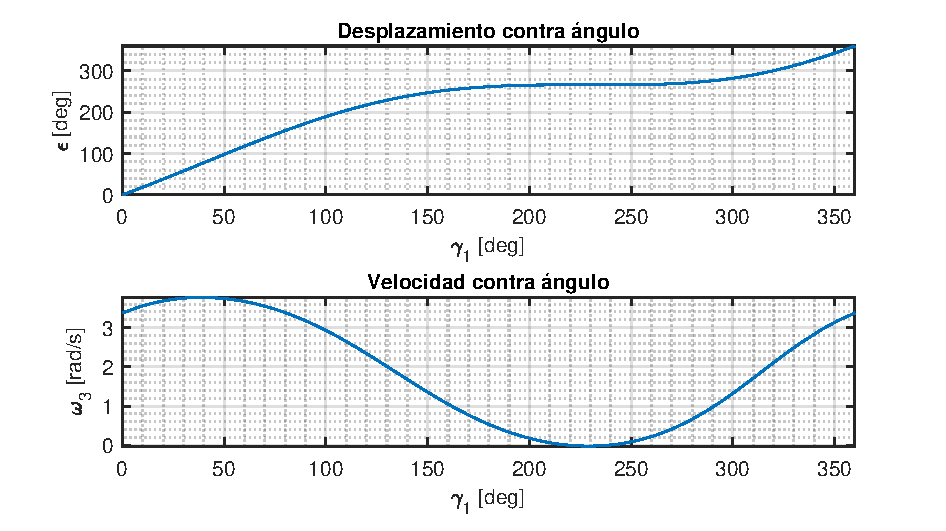
\includegraphics[width=\textwidth]{Des_vel_met_trig}
\end{figure}

\newpage
\subsection{Método vectorial}
En el método vectorial las variables son inicializadas de manera diferente, puesto que por la naturaleza del ejercicio es necesario incorporar variables del tipo \textbf{linspace} para que puedan ser calculados de manera correcta, así mismo son generadas las matrices inicializadas con 0. Para el computo no es necesario simplemente usar nuevamente las variables de tipo \textbf{function handler} por lo que el calculo de las ecuaciones esta realizado en las lineas 39 y 41 respectivamente. 

Nuevamente, el mostrado de las graficas se realiza mediante el comando \textbf{plot} que permite imprimir los valores de cada uno de los vectores. 
{\small
\inputminted{matlab}{Codigos/ADA5_metodo_vec.m}}

\begin{figure}[ht]
    \centering
    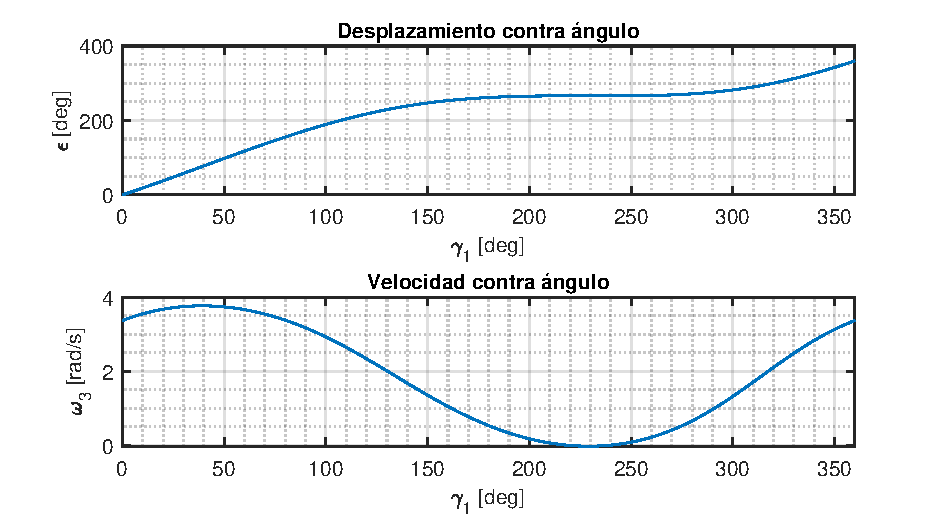
\includegraphics[scale=0.75]{Des_vel_met_vec}
\end{figure}

\newpage
\section{Animación}

Para las animaciones, se empleo el codigo del calculo anterior al que se lea agrego un bucle for, que permitia la generacion de la animación mediante el \textbf{drawnow}. Cada uno de los engranes esta dibujado mediante el comando \textbf{viscircles}, mismo que se utiliza en ambas formas (vectorial, y trigonometrico). 
\subsection{Método trigonométrico}
{\small
\inputminted{matlab}{Codigos/ADA5_metodo_trig_animacion.m}}

\newpage
\subsection{Método vectorial}

{\small
\inputminted{matlab}{Codigos/ADA5_metodo_vec_animacion.m}}

\nocite{*}
\vfill
\bibliographystyle{IEEEtran}
\bibliography{Referencias}

\end{document}